\documentclass{article} % For LaTeX2e

\usepackage{iclr2026_conference,times}

\usepackage{hyperref}
\usepackage{url}
\usepackage{booktabs}
\usepackage{multirow}
\usepackage{amsmath,amssymb}
\usepackage{graphicx}
\usepackage{xcolor}
\usepackage{tikz}
\usetikzlibrary{arrows.meta}
\usepackage{pgfplots}
\pgfplotsset{compat=1.16}
\usepackage{algorithm}
\usepackage{algpseudocode}
\usepackage{enumitem}
\usepackage{caption}
\captionsetup{font=small,labelfont=bf}

\newcommand{\pp}{\,\mathrm{pp}}
\newcommand{\kvm}{VeraKV}

\title{Select, Don't Construct:\\
Verbatim KV-Memory for Long-Horizon Agents}

\author{Zefeng Cai\\
\texttt{3294005475a@gmail.com}}

% Preprint using the ICLR 2026 style; not under review.
\iclrfinalcopy

\begin{document}
\maketitle
\lhead{Preprint}

\begin{abstract}
Long-horizon agents (coding, web, embodied, multi-session chat) accumulate
interaction histories that overflow any context window. Many deployed memory
systems answer this by \emph{constructing} a lossy store---extracting atomic
facts, building knowledge graphs, or summarizing---and retrieving from it; on
dense, objective agent trajectories this destroys exactly the evidence a
question needs. \kvm{} takes the opposite route: \emph{construct indices, not
answer payloads}. It keeps the raw turns, builds only a cheap extractive index
and overview over them, routes each query to the spans it needs, and rehydrates
those spans \emph{verbatim}---a small, readable framework (recency-tiered
verbatim store, pluggable router, verbatim rehydration) for self-hosted
inference.

Our central finding is that \emph{payload fidelity}---not memory construction,
and not router sophistication---is the dominant \emph{memory-side} variable. On
\textbf{AMA-Bench} (official Qwen3-32B harness, full 2{,}496 QA), under the
harness's \emph{default} answer prompt, the memory stack alone reaches
$\mathbf{0.5954}$: above the purpose-built AMA-Agent ($+2.3\pp$), with every
prior memory system $+10$--$35\pp$ behind. A disclosed, separately ablated
structured answer instruction---a reader-side variable, not a memory
effect---brings the end-to-end recipe to $0.6466$ in our run (submitted for
official leaderboard verification). A same-batch memory$\times$reader
factorial and matched payload ablations locate the gains: re-encoding the
\emph{same} selected evidence lossily costs $5$--$14\pp$ (the poison is
paraphrase, not compression); router sophistication is second-order and
regime-dependent; and the largest single knob is the \emph{reader} instruction
($+5.1$--$5.8\pp$ at either router---decomposed below into an
answer-completeness constant plus a net-zero reasoning trade)---so memory
comparisons that do not control the reader largely measure reader
differences. The same
fidelity-over-lossy-payload pattern holds on \textbf{LOCOMO} and
\textbf{LongMemEval-S}.

Because the store is verbatim KV, selection is also a \emph{serving} primitive:
prefill the trajectory once, gather the selected spans' cached KV at their
original positions, and re-prefill only the question---faithful to a
full-prefill-then-mask oracle in our tests, and $1.6$--$10.9\times$ faster to
first token as the selected evidence grows. We scope this precisely: the
accuracy results above use the text-assembly pipeline; KV sub-selection is its
serving-layer equivalent, validated for parity on real trajectories (a
prototype microbenchmark; decode still attends over the selected KV).

The recipe wins when history overflows the window or distractors drown the
reader; full context can win when it fits, and construction-time extraction can
win for a weak reader on tiny isolated facts. We map these boundaries and
release code, configurations, prompts, raw predictions, and judge outputs
(\url{https://github.com/oklen/VeraKV}) as a reproducible baseline that centers
payload fidelity over memory construction.
\end{abstract}

\section{Introduction}
\label{sec:intro}

A long-horizon agent's state is its history: the tool calls it issued, the
observations it received, the reasoning it wrote. As that history grows past the
model's context window, the agent needs a memory. The prevailing answer is to
\emph{construct} one---to run an LLM over the trajectory that extracts atomic
facts (Mem0~\citep{mem0}), writes and links notes (A-Mem~\citep{amem}), distills
hierarchical summaries (MemoryBank~\citep{memorybank}), or builds a temporal
knowledge graph (Zep~\citep{zep})---and then retrieve from that constructed,
lossy store. This is natural for \emph{dialogue} memory, where the salient
content is a handful of stable user facts. It is a poor fit for \emph{agent
trajectories}, where the answer is often an exact value, a step index, a code
diff, or an SQL filter that a fact-extractor paraphrases away. AMA-Bench
\citep{amabench} makes this concrete: purpose-built dialogue-memory systems
(Mem0 $0.21$, A-Mem $0.32$, MemGPT $0.33$, MemoryBank $0.34$) all score
\emph{below} a no-memory long-context baseline ($0.52$) on dense agent
trajectories---lossy construction is the bottleneck.

Our claim is a positioning one: for these workloads, a deliberately simple
alternative to construction is surprisingly strong. A KV cache built over the full
trajectory is already a usable associative memory of it; the operation we want is
not to compress it but to \emph{select} which raw spans a query needs and to
\emph{rehydrate them verbatim}. Algorithmically this is close to query-aware
raw-chunk retrieval; the contribution is the empirical case that raw-span memory
beats constructed memory on agent trajectories, plus the systems mechanism that
makes it cheap. Selection denoises (it drops
the irrelevant turns that drown the answer) while preserving the exact tokens
that construction would lose, and it is cheap to deploy on self-hosted inference
(vLLM~\citep{vllm}, SGLang~\citep{sglang}) because the query-independent part of
the context is prefilled once and reused. The claim is deliberately
conditional, and we keep it so throughout: \emph{select verbatim} when the
history overflows the window or distractors drown the reader; \emph{full
context} can win when it fits and the reader can exploit it;
\emph{construction-time extraction} wins only for a weak reader over tiny
isolated facts (\S\ref{sec:limits}).

We build this into \kvm{} (\S\ref{sec:method}) and evaluate it on three benchmark
families (\S\ref{sec:results}). Our contributions:

\begin{enumerate}[leftmargin=2em,itemsep=2pt]
\item \textbf{A finding with design consequences: payload fidelity dominates}
(\S\ref{sec:ama}, \S\ref{sec:analysis}). Selecting raw spans and re-injecting
them \emph{verbatim} beats every published lossy-construction system by
$+10$--$35\pp$ cross-system, and matched-evidence ablations make the payload's
role causal: re-encoding the \emph{same} selected evidence as summaries or
facts costs $8$--$14\pp$ in a stripped oracle setting and $5$--$6\pp$ inside the
deployed pipeline, while a deterministic swap to the \emph{original lines} of
the same steps costs only $2.6\pp$---the cost is paraphrase, not compression.
\item \textbf{A memory$\times$reader confound audit} (\S\ref{sec:analysis}): a
same-batch factorial separates memory-side from reader-side gains---routing
refinements are second-order ($+1.4\pp$ semantic / $+1.7\pp$ structural on AMA;
regime-dependent: $+4.3\pp$ on LongMemEval, $+12.6\pp$ on LOCOMO) while a
one-sentence reader instruction is worth $+5.1$--$5.8\pp$ at either
router---plus a fourteen-mechanism reader-side stress test showing the memory
side \emph{saturates} once routing reaches $\sim\!100\%$ recall.
\item \textbf{Results on official harnesses} (\S\ref{sec:ama},
\S\ref{sec:locomo}, \S\ref{sec:lme}): $\mathbf{0.5954}$ under the AMA-Bench
\emph{default} reader---the memory-side result, above the purpose-built
AMA-Agent---and $0.6466$ end-to-end with the separately ablated reader
instruction, on our run of the official harness over the full 2{,}496 QA
(above the prior leaderboard best $0.6246$; submitted for official
verification); competitive LOCOMO ($0.704$ vs Mem0 $0.671$\,/\,Zep $0.660$ under the
public protocol, positioned as an out-of-domain check); LongMemEval-S within a
stated regime boundary.
\item \textbf{A serving mechanism: literal KV sub-selection} (\S\ref{sec:eff}):
selected spans are served by gathering their cached KV at original positions,
not re-encoded. It reproduces a full-prefill-then-mask oracle ($100\%$
first-token argmax on synthetic and real AMA trajectories, and on a non-Qwen
backbone), is accuracy-neutral vs the text pipeline on real AMA (tied within
noise under a consistent reader/judge), and runs $1.6$--$10.9\times$ faster to
first token as selected evidence grows (prototype microbenchmark), on top of
$\sim$2M prefill tokens saved per full AMA run.
\item \textbf{A regime map and a forkable baseline} (\S\ref{sec:method},
\S\ref{sec:limits}): a small, readable framework, plus quantified boundaries
for the conditional claim above---when selection wins, when full context does,
when construction does.
\end{enumerate}

\section{Method: \kvm{}}
\label{sec:method}

\kvm{} is a KV-cache memory manager for self-hosted long-horizon agents. The
design goal is a \emph{readable} base others can fork: keep raw context as
reusable KV and select per query, instead of lossily compressing
(Figure~\ref{fig:arch}). Algorithm~\ref{alg:kvm} gives the build-once /
retrieve-per-query loop and Table~\ref{tab:config} its default configuration;
every row of that table is a swap point, and the paragraphs below walk the
components in turn.

\begin{figure}[t]
\centering
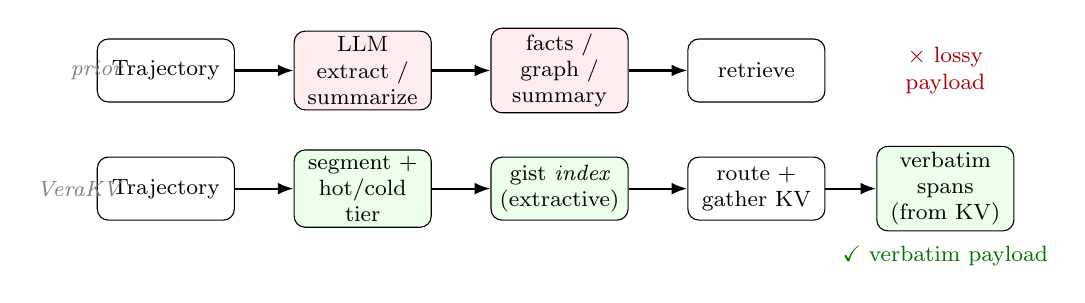
\begin{tikzpicture}[font=\footnotesize,
  b/.style={draw, rounded corners, align=center, text width=16mm, minimum height=8mm, inner sep=2pt},
  L/.style={b, fill=red!7}, G/.style={b, fill=green!8},
  a/.style={-{Latex[length=2mm]}, thick}]
 % Traditional (top)
 \node[b] (t1) at (0,1.5) {Trajectory};
 \node[L] (t2) at (2.5,1.5) {LLM extract / summarize};
 \node[L] (t3) at (5.0,1.5) {facts / graph / summary};
 \node[b] (t4) at (7.5,1.5) {retrieve};
 \node[align=center] at (9.9,1.5) {\textcolor{red!70!black}{$\times$ lossy}\\\textcolor{red!70!black}{payload}};
 \draw[a] (t1)--(t2); \draw[a] (t2)--(t3); \draw[a] (t3)--(t4);
 \node[anchor=east, gray] at (-0.4,1.5) {\textit{prior}};
 % Ours (bottom)
 \node[b] (o1) at (0,0) {Trajectory};
 \node[G] (o2) at (2.5,0) {segment + hot/cold tier};
 \node[G] (o3) at (5.0,0) {gist \emph{index} (extractive)};
 \node[b] (o4) at (7.5,0) {route + gather KV};
 \node[G] (o5) at (9.9,0) {verbatim spans (from KV)};
 \draw[a] (o1)--(o2); \draw[a] (o2)--(o3); \draw[a] (o3)--(o4); \draw[a] (o4)--(o5);
 \node[anchor=east, gray] at (-0.4,0) {\textit{\kvm{}}};
 \node[green!45!black] at (9.9,-0.85) {\checkmark\ verbatim payload};
\end{tikzpicture}
\caption{Prior memory systems \emph{construct} a lossy store (extract/summarize/
graph) and retrieve from it. \kvm{} keeps raw segments, builds only a cheap
\emph{extractive} gist index over the cold ones, and at query time routes to and
\emph{gathers the selected spans' KV} verbatim---gist routes, verbatim answers.}
\label{fig:arch}
\end{figure}

\paragraph{Segments and three recency tiers.}
The trajectory is flattened into \texttt{Segment}s (for agent traces, one per
turn: \texttt{action}\,/\,\texttt{observation}; for dialogue, one per
utterance/session with its timestamp). At query time the segments occupy three
tiers. \textbf{Hot}: the most recent segments, kept \emph{verbatim} (a recency
prior). \textbf{Warm}: older segments \emph{rehydrated verbatim} when the router
selects them for the current query. \textbf{Cold}: every other old segment,
represented by a lightweight \emph{gist}---a cheap \emph{extractive} snippet
(the head of the action/observation), \emph{not} an LLM summary. The gist plays
two roles: it is the \emph{routing index}, and in the assembled context each
un-selected cold turn appears only as its one-line gist inside a recency
\emph{overview}---navigation scaffolding, so the reader can see the shape of the
whole trajectory. The answer-bearing content is served \emph{verbatim}: recent
turns in full, plus the router-selected turns rehydrated in full as an appendix.
Any turn the query actually needs is thus upgraded to verbatim; a gist is never
the payload for selected evidence. Even the index is non-generative: we
\emph{construct for indexing and scaffolding} but \emph{answer from verbatim}.
The slogan is \emph{gist routes, verbatim answers}. Both halves of this layout
earn their tokens: cutting the overview collapses narrative-heavy domains
($-27\pp$ on \textsc{Embodied} in the budget sweep of \S\ref{sec:analysis}),
while answering \emph{from} lossy re-encodings instead of verbatim spans costs
$8$--$14\pp$ (Fig.~\ref{fig:payload}).

\paragraph{The router (pluggable; its payoff is regime-dependent).}
A \texttt{Router.select(query, candidates, k)} interface returns which old
segments to rehydrate. In order of cost: \textbf{Lexical} (token overlap,
BM25-like; free, zero-dependency, already strong); \textbf{Embedding} (dense
retrieval with a lexical pre-filter to bound cost); \textbf{Hybrid}
(reciprocal-rank fusion of the two, which tops both components); and a
\textbf{step-pinning} variant that additionally pins the steps a question names
(``step $N$'', turn references)---a cheap \emph{structural} cue, not a fancier
scorer. We view step-pinning as a minimal instance of \emph{structural address
resolution}: agent trajectories are not unstructured documents but event logs
with stable addresses (step and turn indices, tool-call ids, file paths, URLs),
and when a query names an address the memory should \emph{dereference} it
deterministically---reserving content-based routing for the remaining
budget---rather than force all access through semantic similarity. The address
inventory is measured, not assumed: $82\%$ of AMA-Bench questions carry at
least one deterministically dereferenceable address (step/turn indices $73\%$,
quoted literals $35\%$, code identifiers $10\%$, file paths $6\%$; analysis
script released), so step indices are the most \emph{common} address type, not
the only one---our pin implements that type, and its contribution is reported
separately throughout (\S\ref{sec:analysis}). How much
router sophistication helps is regime-dependent (\S\ref{sec:analysis}); on
step-indexed agent trajectories a cheap router already saturates, and the
verbatim \emph{substrate} does the work.

\paragraph{Verbatim rehydration is the substrate.}
Selected segments are rehydrated \emph{byte-for-byte}, not summarized. Lossy
construction destroys dense objective information (exact values, code, IDs);
verbatim selection avoids that and, by dropping irrelevant turns, also denoises
relative to dumping the full context (lost-in-the-middle). Under a hard budget, a
query-focused per-step trim keeps only the query-relevant \emph{lines} of a giant
observation---a rule/lexical line filter that preserves the original lines
verbatim (no paraphrase)---letting more of a multi-hop chain fit. This trim
fires only when a single observation overflows the budget; because it removes
surrounding lines, it can drop context a question needs (e.g.\ in a stack
trace, diff, or DOM), a failure mode we flag. ``Verbatim'' therefore means
\emph{retained evidence is verbatim}, not \emph{the full observation is always
retained}.

\paragraph{KV reuse by sub-selection (the efficiency claim).}
Because the store is verbatim KV, selection is a \emph{cache} operation, not a
prompt operation. We prefill the episode's trajectory once into a key--value
cache, recording each segment's token span. At query time the router names the
segments to keep; we \emph{gather their cached KV at the original positions}
(position-preserving, so RoPE encodes the true inter-span distances---renumbering
would require re-rotating the stored keys) and decode the question on top,
\emph{re-prefilling nothing but the question itself}. The selected verbatim spans
are thus served from the cache, never re-encoded. Because RoPE is relative,
keeping spans at their original positions is exact for the retained-and-earlier
tokens: this sub-selected prefill agrees with a full-prefill-then-mask-dropped
oracle on the first decoded token in our checks (\S\ref{sec:eff}). The
per-query \emph{prefill} is therefore $O(\text{question})$ rather than
$O(\text{selected evidence})$---the selected spans are not re-encoded, though the
decode still attends over their KV---so the more a multi-hop query pulls, the
larger the prefill saving. Self-hosting gives full control of this reuse;
a prefix-friendly layout additionally benefits from the prompt-caching that
production APIs now expose.

\paragraph{Assembly: two modes.}
The deployed \emph{benchmark (text) pipeline} assembles three blocks,
$[\,\text{overview}\,\Vert\,\text{selected turns}\,\Vert\,\text{question}\,]$
(selected warm turns verbatim), where the overview $=$ hot turns verbatim $+$
every cold turn as its one-line gist. The overview is query-independent
(identical for every query in an episode, so its KV is prefilled once and
reused); the evidence appendix and question vary per query. \emph{All headline
benchmark numbers use this layout}; the budget sweep and gist-only ablations
(\S\ref{sec:analysis}) probe its two halves. The \emph{compact KV-serving mode}
evaluated in \S\ref{sec:eff} drops the overview and serves $[\,\text{selected
turns in temporal order}\,\Vert\,\text{question}\,]$ (hot $+$ router-selected
warm, all verbatim, no gist), gathering the selected spans' cached KV at their
original positions. In both modes every turn keeps its explicit \texttt{<step
$N$>} tag, so the reader reconstructs the timeline from tags rather than
physical position: selecting a subset in temporal order does not scramble
temporal reasoning, and the recent (hot) turns are never displaced by older
selected ones. The cacheable object is \emph{not} a fixed text prefix---the
selected set varies per query---but the one-time trajectory prefill, from which
each query gathers its spans' KV at their original positions (\S\ref{sec:eff});
a hosted API additionally reuses the stable
$[\,\text{system}\,\Vert\,\text{task}\,]$ header via contiguous-prefix caching.

\paragraph{Answer prompt.}
The reader answers over the assembled context with a fixed prompt; we evaluate
both the harness default and a one-sentence structured instruction, and report
them as a separately ablated \emph{reader-side} variable throughout
(\S\ref{sec:analysis}).

\paragraph{What it is not.}
Not a lossy fact/graph/summary memory (we keep raw spans); not a KV
eviction/compression scheme (we select and rehydrate at full precision); its
arbitrary-span KV reuse is realized self-hosting, though the prefix-friendly
layout also benefits hosted prompt-caching.

\begin{algorithm}[t]
\caption{\kvm{}: build once, retrieve (and gather KV) per query. In the KV path,
un-selected turns are \emph{masked from the query's attention}, not re-encoded
away: the retained spans' KV was computed in their presence, a carryover we
measure and bound in \S\ref{sec:eff} and \S\ref{sec:limits}.}
\label{alg:kvm}
\begin{algorithmic}[1]
\Procedure{BuildMemory}{trajectory $T$}
  \State segment $T$ into turns; store each raw payload $s_i$ (action/observation) \emph{verbatim}
  \State for each $s_i$: $\mathrm{gist}_i \gets \textsc{ExtractHead}(s_i)$ \Comment{cheap extractive index, not an LLM summary}
  \State prefill the flattened $T$ once into KV cache $C$; record each $s_i$'s token span
  \State \Return $(\{s_i\},\{\mathrm{gist}_i\}, C, \mathrm{spans})$
\EndProcedure
\Procedure{Retrieve}{query $q$, budget $B$}
  \State $H \gets$ the $h$ most recent turns (hot tier, kept verbatim)
  \State $P \gets$ turns named by structural refs in $q$ (``step $N$'', ``turns $N$--$M$'')
  \State score the remaining (cold) turns by router $R(q,\cdot)$ \Comment{lexical / embedding / RRF hybrid}
  \State $K \gets$ top-$k$ of $P \cup \mathrm{scored}$ under budget $B$; line-trim oversized turns if needed
  \State \textbf{gather} $C$'s KV for $H \cup K$ at their \emph{original} positions (position-preserving)
  \State decode $q$ over $[\,H\,\Vert\,K\,]$ verbatim, re-prefilling only $q$ \Comment{un-selected turns masked, not erased}
\EndProcedure
\end{algorithmic}
\end{algorithm}

\begin{table}[t]
\centering
\caption{\kvm{} default configuration (the fork surface; every row is swappable).}
\label{tab:config}
\footnotesize
\begin{tabular}{ll}
\toprule
Component & Default setting \\
\midrule
Hot tier & $h{=}4$ most recent turns, verbatim \\
Cold gist & extractive head: \texttt{action[:120]} $+$ \texttt{obs[:160]} chars (no LLM) \\
Lexical router & token overlap (BM25-like) over \texttt{[a-z0-9]+}, zero-dependency \\
Embedding router & Qwen3-Embedding-0.6B, cosine top-$k$, lexical pre-filter \\
Hybrid router & RRF of \{lexical, embedding\}, $c{=}60$, $4k$ candidates per sub-router \\
Step-pin & regex \texttt{(turn|step)s?\,$N$(--$M$)?}; pin named turns verbatim \\
Rehydration $k$ & top-$5$ selected turns (budget-bounded) \\
Context budget & 22k (32k window $-$ 10k thinking reserve); truncate oldest first \\
Answer prompt & structured: sub-questions $\rightarrow$ cite evidence $\rightarrow$ compose (App.~\ref{app:instr}) \\
Reader / judge (AMA) & Qwen3-32B (official Track B; LOCOMO/LME: \S\ref{sec:setup}) \\
\bottomrule
\end{tabular}
\end{table}

\section{Experimental setup}
\label{sec:setup}

We evaluate on three long-term-memory families that stress different inputs:
\textbf{AMA-Bench}~\citep{amabench} (agent execution trajectories),
\textbf{LOCOMO}~\citep{locomo} (multi-session dialogue), and
\textbf{LongMemEval-S}~\citep{longmemeval} (long-context chat-assistant
histories). Unless noted, the reader and the LLM-as-judge are the same model as
each benchmark's official protocol, and we report each benchmark's own metric.

For AMA-Bench we run the \emph{official} \texttt{run.py} harness end to end
(memory construction $\to$ per-query retrieval $\to$ answer $\to$ LLM-as-judge) on
the full open-ended set (208 episodes / 2{,}496 QA, six domains), with backbone
\emph{and} judge both Qwen3-32B~\citep{qwen3} (the official ``Track B''), so our
numbers drop directly into the published table; context is capped at 22k tokens
(the 32k window minus the thinking reserve). For LOCOMO we report both the public
gpt-4o-mini leaderboard protocol (comparable to Mem0/Zep) and a consistent-judge
regime (reader = judge = Qwen3-32B) that removes the cross-paper judge confound.
For LongMemEval-S we report only the Qwen3-32B target-reader regime
(\S\ref{sec:limits} explains the scoping).

\section{Results}
\label{sec:results}

\subsection{AMA-Bench: leading results on agent-trajectory memory}
\label{sec:ama}

Table~\ref{tab:ama} places \kvm{} on the AMA-Bench leaderboard. With only a
\emph{free lexical} router, \kvm{} already matches the purpose-built AMA-Agent
($0.5621$ vs $0.5722$) and beats every other published memory system by $+10$ to
$+35\pp$---confirming the core thesis that verbatim selection over raw turns is a
stronger substrate than lossy construction or similarity retrieval. Memory-side
improvements alone---the hybrid router plus the structural step-pin
(\S\ref{sec:analysis}), still under the harness's \emph{default} answer
prompt---reach $0.5954$, $+2.3\pp$ above AMA-Agent ($95\%$ bootstrap CI
$[0.576,0.615]$ over QA; $[0.571,0.620]$ under the more conservative
episode-cluster resampling, whose lower bound sits marginally below AMA-Agent's
$0.5722$---we therefore claim ``above'', not ``significantly above''). Our headline
run additionally swaps the reader's one-sentence answer instruction for a
structured one (``break the request into sub-questions, answer each citing exact
evidence verbatim, then give the final answer''; all three instructions we run
are reproduced verbatim in Appendix~\ref{app:instr}), which we disclose and
ablate as a \emph{reader-side} variable, orthogonal to the memory
(\S\ref{sec:analysis}):
with it, \kvm{} reaches \textbf{0.6466} on our run of the official harness,
above AMA-Agent ($+7.4\pp$) and the prior (unreleased) leaderboard best,
HybridFocus $0.6246$ (submitted for official leaderboard verification; we
release configs, raw predictions, judge outputs, and the submission file
itself). AMA-Bench ships only a test split, so---for every system on the leaderboard
alike---tuning necessarily happened on it; we disclose our tuning surface
exactly. It consists of a handful of discrete choices, each ablated in this
paper: the router (three candidates; Table~\ref{tab:ablation}), the answer
instruction (two candidates, both verbatim in Appendix~\ref{app:instr}), and
the structural step-pin (on/off, with corruption controls). The context budget
is forced by the model window (and swept in \S\ref{sec:analysis}); the
remaining knobs (hot tier $h{=}4$, top-$k{=}5$, gist head lengths) are the
framework's defaults and were never searched. The full configuration is frozen
in the released repository, and runs after the freeze are ablations, not
tuning. Our defense against overfitting is this small, disclosed, discrete
surface plus consistency across three benchmark families---not a held-out
split that does not exist. Per domain (Table~\ref{tab:ama-domain}) \kvm{} beats AMA-Agent in five of
six domains; the exception is \textsc{Software}, which we dissect below.

A faithful re-run of the full harness reproduces this headline ($0.643$ under the
Qwen3-32B judge; $95\%$ bootstrap CI $[0.623,0.662]$ over the $2{,}496$ QA), and
addresses the natural worry that a Qwen reader graded by a Qwen judge inflates the
score. Re-judging that run's \emph{identical} predictions with an independent
Llama-3.1-70B judge---a different model family---yields $0.677$ $[0.658,0.695]$ with
$84\%$ item-level agreement: on our predictions, the Qwen judge is the stricter of
the two. We note the official AMA-Bench documentation reports a \emph{leniency}
bias for Qwen3-32B as a judge in absolute terms; since every leaderboard system is
scored by the same judge, our \emph{comparisons} are on equal footing, and we
treat the cross-family re-judge as supportive rather than definitive. The per-type gap is concentrated where the
reader, not the router, is the bottleneck: on \textsc{Software} the accuracy drop is
uniform across question types ($0.37$--$0.61$), and two probes pin the cause down.
First, \emph{recall}: on all $268$ step-referencing \textsc{Software} questions the
asked step is present in the selected context ($100\%$), and every error is a
reader-side failure. Second, \emph{access}: giving the reader deterministic lookup
tools over the lossless store (exact get-by-index, exhaustive search) leaves
accuracy unchanged ($+0.7\pp$, same-batch; \S\ref{sec:analysis}). Third,
\emph{format}: forcing the reader to answer by \emph{copying} exact strings
verbatim (a quote-first instruction) makes things far worse ($-10.0\pp$,
$0.363$ vs $0.463$, same batch)---suppressing the reader's own reasoning costs
much more than paraphrase penalties ever did. Fourth, \emph{process}: we gave
our single-pass reader that loop---up to four ReAct rounds of deterministic
lookups over the lossless store with a running investigation transcript (no
code execution). Letting the loop \emph{replace} the answering pass costs
$-9.0\pp$ (same batch); restricting it to \emph{evidence-gathering}, with the
answer still produced by the structured single pass, changes nothing
($0.4676$ vs control $0.4676$, $\pm0.0\pp$). So the gap is not retrieval, not
access, not answer formatting, and not prompted iteration either. What remains
unique to AMA-Agent's answer production is \emph{executing code over the full
trajectory}---computing counts, diffs, and aggregations rather than reading
them---plus its construction-time causal index. The
reasoning-heavy residue is the same failure mode we quantify on LongMemEval
(\S\ref{sec:lme}), where $91\%$ of the router's misses are reasoning failures
with the gold evidence already in context. We treat this as a complementary
paradigm, not a deficiency the memory can absorb (\S\ref{sec:limits}).

\begin{table}[t]
\centering
\caption{AMA-Bench, average accuracy over the full 2{,}496 QA (Qwen3-32B backbone
and judge, official harness). Baseline rows are the published AMA-Bench numbers;
\kvm{} rows are our runs on the same harness, labeled with the answer prompt they
use (default vs the disclosed structured instruction, \S\ref{sec:analysis}) so
memory-side and reader-side effects stay separable in the table itself; the
$0.6466$ run is submitted for official leaderboard verification.}
\label{tab:ama}
\small
\begin{tabular}{lc}
\toprule
Method & Avg.\ accuracy \\
\midrule
\textbf{\kvm{} (hybrid$+$pin memory, structured reader)} & \textbf{0.6466} \\
HybridFocus (prior leaderboard best, unreleased) & 0.6246 \\
\kvm{} (hybrid$+$pin memory, \emph{default} reader) & 0.5954 \\
AMA-Agent (purpose-built) & 0.5722 \\
\kvm{} (lexical router, default reader) & 0.5621 \\
\midrule
MemoRAG~\citep{memorag} & 0.4606 \\
HippoRAG2~\citep{hipporag} & 0.4480 \\
BM25 & 0.3436 \\
MemoryBank~\citep{memorybank} & 0.3397 \\
MemGPT~\citep{memgpt} & 0.3304 \\
A-Mem~\citep{amem} & 0.3186 \\
Mem0~\citep{mem0} & 0.2104 \\
\midrule
Long-context Qwen3-32B (no memory) & 0.52 \\
\bottomrule
\end{tabular}
\end{table}

\begin{table}[t]
\centering
\caption{AMA-Bench per-domain accuracy: \kvm{} (hybrid$+$pin memory,
structured reader---the $0.6466$ run) vs the purpose-built AMA-Agent. \kvm{}
wins five of six domains.}
\label{tab:ama-domain}
\small
\setlength{\tabcolsep}{4pt}
\begin{tabular}{lcccccc}
\toprule
& TEXT2SQL & SOFTWARE & WEB & GAME & EMBODIED & OPENWORLD \\
\midrule
\kvm{} (pin) & \textbf{0.740} & 0.475 & \textbf{0.694} & \textbf{0.683} & \textbf{0.575} & \textbf{0.681} \\
AMA-Agent    & 0.609 & \textbf{0.636} & 0.517 & 0.644 & 0.499 & 0.471 \\
\bottomrule
\end{tabular}
\end{table}

\subsection{LOCOMO: competitive with dedicated dialogue-memory systems}
\label{sec:locomo}

On LOCOMO's public protocol (reader = judge = gpt-4o-mini, the Mem0/Zep
convention), \kvm{}'s compact hybrid-retrieval arm reaches $J=0.704$, beating
Mem0 ($0.671$) and Zep ($0.660$)---though under this same gpt-4o-mini judge
\emph{full-history prompting} scores higher still ($0.756$), so we do not claim to
beat full context here. The two judges disagree on exactly that comparison, which is
why we re-run it under a single consistent reader/judge (Qwen3-32B, which removes
the cross-paper judge confound): there, compact selection \emph{does} edge out
full-history prompting ($0.716 > 0.661$), because dropping the irrelevant
turns denoises---note a full-history prompt is not an oracle, since it carries the
distractors that hurt the reader. Verbatim memory also abstains correctly on the adversarial,
unanswerable category $87$--$89\%$ of the time (vs $75\%$ for full context),
because it knows whether evidence exists.

We position LOCOMO as an \emph{out-of-domain sanity check}, not a headline
claim: the benchmark has known protocol variants (QA subsets, judge choices),
and newer file- and tool-based systems report stronger numbers under their own
setups (e.g.\ filesystem-backed agents at $0.740$~\citep{lettafiles} and
$0.744$~\citep{pamlocomo}). The useful signal for our thesis is narrower and
survives those caveats: under one fixed protocol, compact verbatim selection is
competitive with dedicated dialogue-memory systems, and under a consistent
judge it beats prompting the full history---on \emph{dialogue}, the workload
construction was designed for.

\begin{table}[t]
\centering
\caption{LOCOMO. Left: public gpt-4o-mini protocol (comparable to Mem0/Zep).
Right: consistent Qwen3-32B judge. ``Full-history'' prompts the entire dialogue
(distractors included); it is a strong baseline, not a gold-evidence oracle.}
\label{tab:locomo}
\small
\begin{tabular}{lc@{\hskip 2.5em}lc}
\toprule
\multicolumn{2}{c}{Public (gpt-4o-mini)} & \multicolumn{2}{c}{Consistent judge (Qwen3-32B)} \\
System & $J$ & Arm & $J$ \\
\midrule
Full-history prompt & 0.756 & \kvm{} (hybrid retrieval) & \textbf{0.716} \\
\textbf{\kvm{} (hybrid retrieval)} & \textbf{0.704} & Full-history prompt & 0.661 \\
Mem0~\citep{mem0} & 0.671 & \kvm{} (lexical retrieval) & 0.590 \\
Zep~\citep{zep} & 0.660 & & \\
\bottomrule
\end{tabular}
\end{table}

\subsection{LongMemEval-S: generalization with a clear boundary}
\label{sec:lme}

LongMemEval-S puts each question over its own $\sim$115k-token, $\sim$50-session
haystack; we evaluate the \emph{full} $500$ questions ($470$ answerable $+\,30$
abstention), with $95\%$ bootstrap CIs, on the official
\texttt{longmemeval\_s} release (xiaowu0162/longmemeval; the benchmark's
oracle evidence-session labels are used \emph{only} for error attribution
between selection and reader failures, never by the method; exact file and
access date ship with our artifacts). In the Qwen3-32B regime two facts hold.
(i) When the history \emph{exceeds} the window---the operative case for long-horizon
agents---the full arm must truncate, and routed selection at a fraction of the budget
beats it decisively: $0.496\,[0.453,0.543]$ vs $0.302\,[0.262,0.343]$ at a 28k budget
($+0.194\,[0.149,0.238]$). The mechanism is clean: truncation drops old evidence
sessions ($95\%$ of its answerable misses are \emph{selection} failures), whereas the
router keeps the gold session in budget ($9\%$ selection-fail). (ii) When the history
instead \emph{fits} an extended 128k window (via YaRN), full context wins overall
($0.564\,[0.519,0.609]$ vs $0.496$; $+0.068\,[0.019,0.119]$)---but at $4.5\times$ the
context, and its edge is confined to \emph{recall/breadth}: full leads on single-session
recall (ss-user $0.828$ vs $0.609$, ss-asst $0.946$ vs $0.768$) and multi-session
($0.405$ vs $0.322$), while routed selection \emph{wins} temporal-reasoning ($0.331$ vs
$0.291$) and knowledge-update ($0.736$ vs $0.708$; Fig.~\ref{fig:lme}). So
``selection $\geq$ full'' is \emph{regime-dependent}, and we state the crossover rather
than cherry-pick a side. Here the router \emph{is} load-bearing (unlike on AMA): the
dense-embedding hybrid beats a lexical router ($0.496$ vs $0.453$; $+0.043\,[0.006,0.079]$),
entirely by cutting selection failures ($9\%$ vs $23\%$).

\begin{figure}[t]
\centering
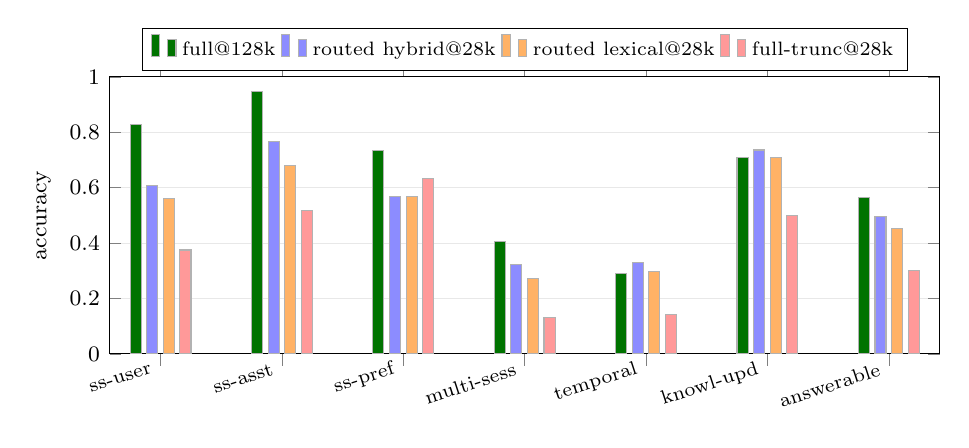
\begin{tikzpicture}
\begin{axis}[
  ybar, bar width=4pt,
  width=\linewidth, height=5.1cm,
  ylabel={accuracy}, ymin=0, ymax=1.0,
  symbolic x coords={ss-user,ss-asst,ss-pref,multi-sess,temporal,knowl-upd,answerable},
  xtick=data, x tick label style={font=\scriptsize, rotate=18, anchor=east},
  legend style={font=\scriptsize, at={(0.5,1.02)}, anchor=south, legend columns=4},
  enlarge x limits=0.07, ymajorgrids, grid style={gray!18}, font=\footnotesize,
  every axis plot/.append style={draw=black!30},
]
\addplot[fill=green!45!black] coordinates {(ss-user,0.828)(ss-asst,0.946)(ss-pref,0.733)(multi-sess,0.405)(temporal,0.291)(knowl-upd,0.708)(answerable,0.564)};
\addplot[fill=blue!45]        coordinates {(ss-user,0.609)(ss-asst,0.768)(ss-pref,0.567)(multi-sess,0.322)(temporal,0.331)(knowl-upd,0.736)(answerable,0.496)};
\addplot[fill=orange!60]      coordinates {(ss-user,0.562)(ss-asst,0.679)(ss-pref,0.567)(multi-sess,0.273)(temporal,0.299)(knowl-upd,0.708)(answerable,0.453)};
\addplot[fill=red!40]         coordinates {(ss-user,0.375)(ss-asst,0.518)(ss-pref,0.633)(multi-sess,0.132)(temporal,0.142)(knowl-upd,0.500)(answerable,0.302)};
\legend{full@128k, routed hybrid@28k, routed lexical@28k, full-trunc@28k}
\end{axis}
\end{tikzpicture}
\caption{LongMemEval-S per-type accuracy, full $500$ questions (Qwen3-32B served at 128k
via YaRN; internal Qwen3-32B judge; $95\%$ bootstrap CIs on \emph{answerable} in
\S\ref{sec:lme}). Two regimes: when the 115k haystack \emph{fits} the window, full context
wins overall (answerable $0.564$), but routed selection at $4.5\times$ less budget
\emph{leads} on temporal and knowledge-update; at a 28k budget where the history must
truncate, routed selection ($0.496$) beats truncation ($0.302$) by $+19\pp$, and the
embedding-hybrid router beats lexical by $+4\pp$. Correct-abstention (not shown) is
$0.60$/$0.67$/$0.67$/$0.77$.}
\label{fig:lme}
\end{figure}

\subsection{Where the gain comes from: substrate, not router}
\label{sec:analysis}

It would be tempting to credit a clever router. A same-batch
memory$\times$reader factorial (Table~\ref{tab:factorial}) says otherwise. The
verbatim-selection substrate is the hero---\emph{just selecting raw spans}, with a
token-overlap router and the harness's default reader, already matches the
purpose-built system ($0.5601$ vs $0.5722$), and the full memory stack under that
same default reader beats it ($0.5954$, $+2.3\pp$). Routing refinements are
second-order: the dense-embedding hybrid adds $+1.4\pp$ and the structural
step-pin $+1.7\pp$, consistently at either reader ($+3.1$--$3.5\pp$ total). The
single largest effect is not in the memory at all: swapping the reader's
one-sentence answer instruction for a structured one adds $+5.1$--$5.8\pp$ at
either router, and the two axes are additive to within batch noise (same-day
replicate $\pm0.5\pp$). Memory systems ship with very different readers
(AMA-Agent an agentic tool loop, MemGPT its own control loop), so end-to-end gaps
that do not control the reader conflate the two effects; we report them
separately. Router \emph{sophistication} remains regime-dependent
(Table~\ref{tab:router}): its payoff scales with how lexically un-addressable the
evidence is---modest on step-indexed agent trajectories, load-bearing on diffuse
dialogue (where, on LOCOMO, it is the only thing that lifts selection above full
context). This is a sharper and more honest statement than ``the router is the
lever.''

\begin{table}[t]
\centering
\caption{Same-batch memory$\times$reader factorial on AMA-Bench (full 2{,}496 QA,
official harness; $95\%$ QA-level bootstrap CIs; episode-cluster CIs---208
clusters---are $\sim\!30\%$ wider, e.g.\ $[0.571,0.620]$ for the
default-reader memory stack). The two axes are additive to within batch noise:
routing adds $+3.1$--$3.5\pp$ at either reader, and the one-sentence structured
answer instruction adds $+5.1$--$5.8\pp$ at either router. Under the
\emph{default} reader the memory stack alone already scores above the
purpose-built AMA-Agent ($0.5722$). The lexical/default cell is a same-batch
replicate of Table~\ref{tab:ama}'s lexical row ($0.5601$ vs $0.5621$, run on
different days; the $0.2\pp$ gap is within replicate noise).}
\label{tab:factorial}
\small
\begin{tabular}{lcc}
\toprule
Memory configuration & Default answer prompt & Structured answer prompt \\
\midrule
Lexical router & $0.5601\,[0.541,0.579]$ & $0.6154\,[0.595,0.635]$ \\
$+$ hybrid router $+$ step-pin & $0.5954\,[0.576,0.615]$ & $\textbf{0.6466}\,[0.623,0.662]$ \\
\bottomrule
\end{tabular}
\end{table}

\begin{table}[t]
\centering
\caption{Router sophistication (lexical $\to$ dense-embedding hybrid) is
regime-dependent: its payoff grows with how lexically un-addressable the evidence
is.}
\label{tab:router}
\small
\begin{tabular}{lc}
\toprule
Benchmark (evidence style) & $\Delta$ from the hybrid router \\
\midrule
AMA-Bench (step-indexed trajectories) & $+1.4\pp$ \\
LongMemEval-S (long chat) & $+4.3\pp$ \\
LOCOMO (diffuse dialogue) & $+12.6\pp$ \\
\bottomrule
\end{tabular}
\end{table}

\paragraph{Substrate, then structure, then semantics.}
On AMA-Bench specifically, three memory-side effects separate cleanly
(Table~\ref{tab:ablation}). The \emph{substrate}---selecting raw spans at all,
even with a free token-overlap router---is the bulk of the gain, lifting a
lossy-construction field into AMA-Agent territory. Semantic router
\emph{sophistication} (lexical$\to$dense-hybrid) adds a second-order $+1.4\pp$.
The remaining lever is not a smarter scorer but a one-line \emph{structural} cue:
$73\%$ of AMA-Bench questions cite a step index (``at Turn~38'', ``across steps
28--30''), and pinning exactly those steps adds $+1.7\pp$---and does so
\emph{entirely} on the step-citing questions ($+2.5\pp$ on them vs exactly
$+0.0\pp$ on the rest), a clean mechanism signature. We disclose this benchmark
property rather than lean on it silently: on step-indexed agent traces the order
is substrate~$\gg$~semantic router~$\approx$~structure, and the structural pin is
a transparent rule, not a learned exploit.

\paragraph{Is the result a step-citing artifact? (robustness).}
Largely not, and we cross-check with a second judge. Controlling on the same
Qwen3-32B reader and judge over $910$ step-citing questions, routing the question
with its step \emph{number deleted} costs lexical selection only $-0.2\pp$
($28.6\to28.4$)---so selection locates the evidence by content, not by the index---and
a different-family judge (Llama-3.1-8B) re-scoring the same answers agrees ($-1.0\pp$),
so this is not a judge artifact. The cited step is informative \emph{when present}:
pinning it alone reaches $38.5\%$ vs $28.6\%$ for lexical top-$5$ (and $40.1$ vs $36.0$
under the Llama judge---ordering preserved), because it is the correct evidence, not a
numeric shortcut. Corrupting the resolved address completes the picture: shifting
every pin three steps off its target leaves accuracy unchanged ($0.630$ vs
$0.629$, same batch)---the near-miss keeps the referenced neighborhood in context
and content routing independently recovers the exact step---while replacing every
pin with a far-random wrong step costs $-1.8\pp$ ($0.611$), roughly the pin's own
contribution forgone, with content routing holding the floor. Structural address
resolution is thus a cheap redundant guarantee that degrades gracefully under
corruption, not a fragile dependency. We are careful about one boundary: non-step questions remain
answerable but are genuinely harder, and by how much is judge-dependent (within
$-2.4\pp$ of step-citing under the Qwen judge, but $-14.8\pp$ under Llama), so we claim
robustness to the step \emph{cue}---not that non-step questions are equally easy. The
step-pin is thus a transparent bonus on the step-citing subset, not the source of the
result.

\begin{table}[t]
\centering
\caption{AMA-Bench ablation deltas (full 2{,}496 QA, same-batch). The verbatim
substrate carries the result; semantic and structural routing refinements are
second-order; the reader-side answer instruction---listed for scale, and reported
separately because it is \emph{not} a memory effect---is larger than both
combined.}
\label{tab:ablation}
\small
\begin{tabular}{lc}
\toprule
Component & $\Delta$ Avg.\ accuracy \\
\midrule
Substrate: raw spans vs.\ lossy construction (cross-system) & $+10$ to $+35\pp$ \\
\quad\emph{controlled} (same oracle evidence; Fig.~\ref{fig:payload}) & $+8$ to $+10\pp$ \\
Semantic router (lexical $\to$ dense-embedding hybrid) & $+1.4\pp$ \\
Structural step-pin ($+2.5\pp$ on the $73\%$ cited-step questions, $+0.0$ else) & $+1.7\pp$ \\
\midrule
\emph{Reader-side, for scale: structured answer instruction} & $+5.1$--$5.8\pp$ \\
\bottomrule
\end{tabular}
\end{table}

\paragraph{Controlled payload ablation (oracle evidence).}
The cross-system $+10$--$35\pp$ above conflates payload form with chunking, prompt, and budget. We
isolate the payload with a within-system test: on step-citing questions we take the \emph{exact cited
step} as oracle evidence (holding retrieval fixed) and present that same evidence three ways---the raw
\emph{verbatim} step, an LLM \emph{summary}, or LLM-extracted \emph{facts}---to the same Qwen3-32B
reader, prompt, and judge. Only the payload form varies, so the gap is causal (Fig.~\ref{fig:payload}):
verbatim beats an LLM summary by $+10.1\pp$ and extracted facts by $+8.5\pp$ over $910$ QA, widening to
$+14\pp$ on exact-recall (type A) where lossy forms drop the exact value. This is the controlled version
of ``the substrate is the hero'': matched evidence, matched reader, lossy re-encoding \emph{alone} costs
$8$--$14\pp$. To rule out the reader grading its own generations leniently, a \emph{different-family}
judge (Llama-3.1-8B) re-scoring the same answers preserves the ordering---verbatim $34.3\%$ $>$ facts
$30.2\%$ $>$ summary $29.8\%$, still $+4$--$5\pp$---so the verbatim advantage is not a judge artifact.
(These absolute numbers are deliberately \emph{not} comparable to Table~\ref{tab:ama}: in this stripped
setting the reader sees only the single cited step---no overview, no recent turns, no neighbors---on
step-citing questions only.) A \emph{same-pipeline} version closes that gap in scale: keeping the full
deployed context and replacing only the router-selected verbatim appendix with LLM summaries of the same
steps (same QA, overview, router, reader, and judge; the swap fires on $96\%$ of questions) costs
$-5.1\pp$ ($0.578$ vs $0.629$, same-day). Table~\ref{tab:family} completes the family under
same-batch anchors: swapping the appendix to Mem0-style \emph{extracted atomic facts} costs
$-5.9\pp$, and both generative re-encodings score at or \emph{below} serving no appendix at all
(gist-only $-4.3\pp$)---a lossy re-encoding of the selected evidence adds nothing over the one-line
gists already in the overview. The control that separates \emph{compression} from \emph{paraphrase}
is a deterministic swap to the query-relevant \emph{original lines} of the same steps (no LLM, no
rewording): it costs only $-2.6\pp$, roughly a third of the generative cost. The poison is
paraphrase, not compression; in this pipeline the choice is verbatim---whole spans or extracted
original lines---or nothing.

\begin{figure}[t]
\centering
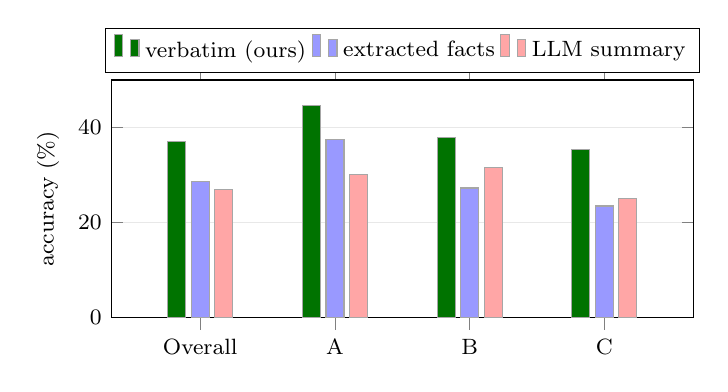
\begin{tikzpicture}
\begin{axis}[
  ybar, bar width=6.5pt,
  width=0.74\linewidth, height=4.6cm,
  ylabel={accuracy (\%)}, ymin=0, ymax=50,
  symbolic x coords={Overall,A,B,C},
  xtick=data,
  legend style={font=\footnotesize, at={(0.5,1.03)}, anchor=south, legend columns=3},
  enlarge x limits=0.22, ymajorgrids, grid style={gray!18}, font=\footnotesize,
  every axis plot/.append style={draw=black!35},
]
\addplot[fill=green!45!black] coordinates {(Overall,37.0)(A,44.6)(B,37.9)(C,35.3)};
\addplot[fill=blue!40]        coordinates {(Overall,28.6)(A,37.4)(B,27.3)(C,23.5)};
\addplot[fill=red!35]         coordinates {(Overall,26.9)(A,30.2)(B,31.6)(C,25.1)};
\legend{verbatim (ours), extracted facts, LLM summary}
\end{axis}
\end{tikzpicture}
\caption{Controlled payload ablation (matched oracle evidence, reader, prompt, and judge;
$910$ step-citing AMA-Bench QA; type A $=$ exact-recall)---only the payload \emph{form}
varies. Re-injecting the selected steps \emph{verbatim} beats lossy re-encodings on every
question type: $+10.1$/$+8.5\pp$ overall over LLM-summary/extracted-facts, widening to
$+14\pp$ on exact-recall. (On the degenerate type D, omitted, all three sit at $\sim\!2\%$.)
Lossy re-encoding of matched evidence \emph{alone} costs $8$--$14\pp$---isolating the substrate.}
\label{fig:payload}
\end{figure}

\begin{table}[t]
\centering
\caption{Same-pipeline payload/layout attribution: each arm differs from the deployed
system \emph{only} in what fills the evidence appendix (or, for the first row, replaces the
assembled context). 1{,}248-QA half, structured reader, 22k budget throughout. $\Delta$ is
against each arm's \emph{same-batch} structured anchor (anchors drift $0.6290\to0.6418$
across days, $\sim$the known 1--2$\pp$ batch noise).}
\label{tab:family}
\small
\setlength{\tabcolsep}{4pt}
\begin{tabular}{lcc}
\toprule
Context / appendix content & Acc & $\Delta$ (same-batch) \\
\midrule
Full trajectory, recency-truncated (no memory) & $0.5577$ & $-8.4\pp$ \\
Appendix $\to$ LLM summaries (same steps) & $0.5777$ & $-5.1\pp$ \\
Appendix $\to$ extracted atomic facts & $0.5825$ & $-5.9\pp$ \\
No appendix (recency$+$gist overview only) & $0.5865$ & $-4.3\pp$ \\
Appendix $\to$ query-relevant \emph{original lines} (no LLM) & $0.6154$ & $-2.6\pp$ \\
Appendix $=$ selected steps verbatim (deployed) & $0.6290$\,/\,$0.6418$ & --- \\
\bottomrule
\end{tabular}
\end{table}

\paragraph{Versus standard vector-RAG.}
The embedding router \emph{is} a standard vector-RAG baseline---it embeds each
step's full text and takes cosine top-$k$, exactly the retrieval stage of
Mem0/A-Mem/AMA-Agent---the only difference being that we re-inject the retrieved
spans \emph{verbatim} rather than a constructed store. On a shared subset its
ordering is $\text{lexical }0.557 < \text{vector-RAG }0.583 < \text{RRF hybrid
}0.600$: our routing edges plain vector retrieval, but all three sit far above
BM25 ($0.3436$) and every lossy-construction system (Table~\ref{tab:ama})---so
``standard RAG with verbatim re-injection'' is already most of the win, and
\kvm{} adds tiering, structural pinning, and KV reuse on top.

\paragraph{Why map the reader axis at all.}
Not to argue for prompt engineering: because any memory comparison that does
not control it is confounded (the factorial above), because the boundary
tells us what a memory should \emph{not} attempt, and because the two axes
are asymmetric in a way that settles design priority---a memory error
(evidence lost to lossy construction or truncation) is unrecoverable
downstream, while every reader-side deficit we found is repairable at answer
time by one sentence or one extra pass. Memory errors are permanent; reader
errors are one sentence away.

\paragraph{Reader-side machinery saturates once routing is strong.}
If a one-sentence reader instruction is worth $+5.5\pp$, is the single-pass
reader leaving more on the table? We stress-tested this with fourteen reader-side
mechanisms over a \emph{fixed} memory (same-batch controls;
Table~\ref{tab:reader}). On the flagship memory: letting the model compress the
selected evidence before answering; a sufficiency gate fused into the answer
prompt that can trigger re-retrieval; the same gate as a separate call; a
query-conditioned entity-state timeline prepended as a scaffold; and
deterministic lookup tools (exact get-by-index, exhaustive search) over the
lossless store. None of these helps; several hurt. The one positive in the
table is re-retrieval under a \emph{weak} (lexical) router ($+1.3\pp$), and the
attribution is exact: the fused gate's $-1.6\pp$ splits into $-2.6\pp$ from the
escape clause perturbing the answer prompt and $+0.4\pp$ from the re-retrieval
action itself. The pattern is uniform: a reader-side
mechanism pays only when it injects information the selected context is actually
\emph{missing}. Once routing reaches $\sim\!100\%$ evidence recall, the memory
side is saturated---residual errors are backbone reading and reasoning failures,
which none of this machinery (including verbatim tool access) repairs.

Four further probes sharpen the law.
\emph{First, the instruction's content cannot be pre-computed.} If a
one-sentence instruction that elicits sub-question reasoning is worth
$+5\pp$, can the memory service cache that reasoning---produce an evidence
plan (sub-questions, cited values, local conclusions) and hand it to a plain
reader? No: prepending such a plan costs $-5.6\pp$ under the default reader
and $-2.7\pp$ under the structured one (same-batch)---\emph{worse than no
scaffold at all}---and the more reasoning a scaffold carries, the more it
hurts (plan $-5.6$ vs state timeline $-1.6$; compression's $-3.0$ removes
context outright, a different failure). The reader inherits the plan's errors
and skips its own derivation: the instruction's value is eliciting the
reader's \emph{own} reasoning in the answering pass, not the reasoning
content. \emph{Second, the reasoning's presentation cannot be compiled.} We
compiled the same selected verbatim evidence into a reasoning-affordant
view---need-grouped quotes, occurrence lists, timelines, conflict and
missing-evidence panels, with conclusions and instructions expressly
forbidden---and handed it to the \emph{default} reader, targeting exactly the
questions the structured instruction fixes (default-wrong, structured-right;
$n{=}316$), with a same-batch raw-context control and a $299$-question
both-right stability sample. The view recovers nothing beyond the control's
spontaneous-recovery rate ($32.6\%$ vs $32.3\%$; a same-config re-run alone
re-fixes a third of the ``fixed'' set, so per-question flips are dominated by
borderline items) and \emph{breaks} $13.4\pp$ of previously-correct questions,
through mechanisms we verified against raw trajectories: appendix-scoped
absences asserted as data-wide facts, and fabricated citations---one audited
compilation promoted an environment's \emph{available-actions menu} to
executed events, with step numbers and quote marks---which the reader trusts
over the overview it still has. A hardened second iteration (subset-scoped
wording, computed deltas and absence claims forbidden, an explicit
option-vs-event rule, a deterministic verbatim-containment guard) still saw
the guard reject $69\%$ of compilations---instructions alone do not enforce
fidelity---and, deployed on the full $1{,}248$-question half, is exactly null
against its same-batch control ($0.5617$ vs $0.5641$ at a $31\%$ serve rate):
harmless, and worthless. \emph{Fidelity can be guarded; usefulness cannot be
compiled.} In hindsight the boundary could not have held: grouping asserts
relevance, a timeline asserts change, a missingness note asserts
nonexistence---every panel of a compiled view is an implicit conclusion, so a
view compiler is a query-time lossy \emph{constructor}, and the paper's core
claim applies to it recursively (the released paired case study shows wins and
losses flowing through the same mechanisms).

\emph{Third, the instruction's parts cannot be specialized by question type.}
Deterministic routing to purpose-built fragments of it (enumerate-then-count,
ledger-only state reconstruction, verbatim-copy, protective direct
answering---rules derived from an annotated 26-case study of what the
instruction fixes and breaks) scores $-3.0\pp$ overall: the routed classes
lose $-7$ to $-23\pp$ while the untouched-default remainder replicates its
anchor ($-0.3\pp$). The routing \emph{direction} was right---on the questions
the instruction breaks, routed fragments gain $+10.7\pp$---but the exchange
rate is ruinous: within the same classes, the questions the instruction
\emph{fixes} lose $-39\pp$, about ten collateral losses per targeted fix.
Every fragment ablates the full derive$\to$cite$\to$compose loop, which is
exactly how the instruction was quietly winning the body of each class; no
rule precision fixes a treatment whose side effect is removing the cure. (We
did not test additive per-class hints appended to the intact instruction.)
\emph{Fourth, a repair mechanism needs something specific to fetch.}
Re-retrieval cannot fix \emph{breadth} starvation: at a 6k budget (a known
$-9.5\pp$ gap), a separate sufficiency gate fires on $19\%$ of questions yet
recovers nothing ($-0.4\pp$)---the budget cut removes the overview, and
fetching more individual steps does not restore breadth.

The law, final form: \emph{a reader-side mechanism pays only when it
supplies specific, query-addressable information the context is missing, or
when it changes the reply the reader is instructed to produce. The
instruction is the only lever that reaches emission behavior---content
cannot (plans, compiled views, checklists, worksheets), and specialized
fragments of the instruction cannot replace it. Pre-computed reasoning
transfers only as a relayed product whose re-emission is itself
completeness-protected---and that composed relay is the one mechanism that
beats the single pass (below).}

\begin{table}[t]
\centering
\caption{Reader-side mechanisms over a \emph{fixed} flagship memory (AMA-Bench,
same-batch $\Delta$ vs the plain single-pass reader; the plan row reports both
readers: default\,/\,structured). Same-day replicate noise is $\pm0.5\pp$; the
tools and loop rows are probed on the \textsc{Software} domain, where the
mechanisms were hypothesized to matter and whose batch noise is
$\pm4\pp$---so $+0.7$ reads as $\approx\!0$; both loop rows are same-batch
against their own control. Only re-retrieval under a weak router helps---the
one case where the mechanism supplies evidence the selected context is
missing.}
\label{tab:reader}
\small
\begin{tabular}{lc}
\toprule
Reader-side mechanism (memory fixed) & $\Delta$ accuracy \\
\midrule
Model-selected evidence compression & $-3.0\pp$ \\
Entity-state timeline scaffold & $-1.6\pp$ \\
Sufficiency gate fused into the answer prompt & $-1.6\pp$ \\
\quad(escape clause alone $-2.6\pp$; re-retrieval action alone $+0.4\pp$) & \\
Sufficiency gate as a separate call & $\pm0.0\pp$ \\
Deterministic lookup tools over the lossless store & $+0.7\pp$ \\
Iterative lookup loop \emph{replacing} the answering pass & $-9.0\pp$ \\
Iterative lookup loop as evidence-gatherer (answer pass kept) & $\pm0.0\pp$ \\
Type-routed specialized instructions (rules from a 26-case study) & $-3.0\pp$ \\
Pre-computed reasoning plan (memory-side artifact) & $-5.6$ / $-2.7\pp$ \\
Re-retrieval under budget starvation (6k cap, gate fires $19\%$) & $-0.4\pp$ \\
\midrule
Requirements checklist appended to the \emph{context} (instruction untouched) & $-1.8\pp$ \\
Verbatim-evidence worksheet appended (containment guard rejects $74\%$) & $-0.7\pp$ \\
\midrule
Re-retrieval under a \emph{weak} (lexical) router & $+1.3\pp$ \\
\bottomrule
\end{tabular}
\end{table}

The arc's endpoint hands the reader the answer itself---and finally explains
the whole arc. A memory-side call runs the full structured pass at full
budget; with a reasoning model its derivation never leaves the thinking block
($99\%$ of visible artifacts begin with the final answer), so by default only
its \emph{product} is exportable. Relayed to the default reader, that product
barely helps: retention of the structured pass's wins is $0.797$ vs $0.773$
with no artifact---the reader re-derives from scratch past the correct answer
sitting in its own context---and an explicit trust instruction lifts the arm
only to $0.593$, $-4.2\pp$ below running the structured pass in place.
Forcing the \emph{process} out looked worse still: an explicit
visible-derivation format demand (with a schematic few-shot) achieves $99\%$
compliance but costs $-11.8\pp$ $[-14.4,-9.1]$ \emph{answered in place, no
relay involved}. But the cost decomposes, and the decomposition dissolves the
mystery. The demand also compresses the \emph{final answer} (median
$869\to247$ chars); a brevity-only demand with no derivation already costs
$-7.5\pp$ $[-10.1,-4.9]$ (at $389$ chars); re-demanding a complete final
answer under the full export format recovers the loss almost entirely
($-1.1\pp$ $[-3.6,+1.6]$ at $786$ chars, statistically zero); and a
verbose-only control $66\%$ \emph{longer} than the anchor is exactly flat
($+0.2\pp$). Across seven same-batch arms the penalty is monotone in how far
the reply is compressed below the instruction's natural output and flat above
it---and the relay arms' ``irreducible'' friction sits on the same curve
(their readers re-emit at $522$--$666$ chars): the concise re-emission, not
the relay, was the ceiling. What is derivation-specific is only fidelity:
$21\%$ of exported derivations quote the context fully verbatim---a post-hoc
reconstruction from thinking, not a record of it.

Protecting completeness at the relay's second stage closes the arc. With the
reader told to verify the memory service's analysis and give its final answer
\emph{in full}, the trust relay of the structured pass's bare answer reaches
$0.659$ and $0.664$ in two same-batch runs ($+2.4$ $[+0.1,+4.7]$ and $+2.8$
$[+0.7,+5.1]$ over the in-place structured anchor) and $0.663$ on the full
$2{,}496$-QA set ($+1.7$ $[+0.1,+3.3]$ over its same-batch anchor
$0.645$)---the composed system meets, and in each batch nominally exceeds,
the single structured pass. The mechanism splits cleanly on the question
pools: on default-wrong/structured-right questions ($n{=}180$) the relay
retains the structured pass's wins in full ($0.72$--$0.73$, matching the
anchor), and on structured-wrong/default-right questions it \emph{repairs}
part of what the structured pass breaks ($0.51$ vs the anchor's
$0.43$)---the second pass buys genuine error correction. Attribution
controls complete the picture: adding the same completeness demand to the
\emph{default} instruction alone (no structured pass anywhere) recovers the
entire \emph{net} gap ($0.583\to0.632$, tying the structured anchor at
$-0.2\pp$ $[-2.7,+2.3]$)---but with a different profile, still $-7\pp$ behind
on the structured-only wins while keeping $+18\pp$ of the default's advantage
on the questions structured breaks. The structured instruction's celebrated
$+5\pp$ thus decomposes into an answer-\emph{completeness} constant
(transferable to any system by one sentence, which we disclose and urge
leaderboards to fix) plus a reasoning-content \emph{trade} (win the multi-hop
pool, break the over-derivation pool) whose net is $\approx\!0$; the relay is
the one configuration that keeps the trade's wins and refunds part of its
losses. Finally, the completeness lever is \emph{instruction-only}: appending
a requirements checklist or a verbatim-evidence worksheet to the
\emph{context} (memory-side presentation, default instruction untouched)
leaves the reply length unmoved ($348\to353$--$379$ chars) and accuracy null
(Table~\ref{tab:reader})---and the worksheet reprises the fabrication
signature (the containment guard rejects $74\%$ of generated worksheets; the
served remainder scores $-3\pp$ on its own subset). Content cannot reach the
emission behavior that one instruction sentence sets.

\paragraph{How much selected context: fill the budget.}
Within the \emph{routed} context, more is monotonically better up to the
window-forced cap: sweeping the assembled-context budget at fixed routing and
reader gives $0.550$ (6k tokens) $\to$ $0.624$ (14k) $\to$ $0.644$ (22k) on a
1{,}248-QA half (same batch; same-day replicate noise $0.5\pp$). ``Context rot''
does not bite \emph{selected} context at these scales---it bites unselected
history (the $0.52$ no-memory row of Table~\ref{tab:ama}; \textsc{OpenWorld},
where recency-truncated full context scores $0.474$ vs routed $0.629$; and the
same-batch control of Table~\ref{tab:family}, where the raw trajectory
recency-truncated to the \emph{same} 22k budget costs $-8.4\pp$, a larger loss
than any payload degradation)---so the
rule is: select first, then fill the window with what was selected. The
recency$+$gist overview earns its tokens (cutting to 6k costs $-27\pp$ on
\textsc{Embodied} and $-23\pp$ on \textsc{Web}); the one exception is
\textsc{Text2SQL}, which \emph{prefers} compact context ($+1$--$3\pp$ at smaller
budgets), pointing to budget-adaptive routing as an open lever. The converse
ablation removes query-time selection instead: answering from the recency
$+$gist overview \emph{alone} (no verbatim appendix) costs $-4.3\pp$
($0.5865$ vs $0.6290$, same-day)---notably still above every constructed-memory
system, but the routed verbatim appendix clearly earns its keep. Both halves of
the assembled context are load-bearing.

\subsection{Efficiency: KV sub-selection decouples cost from evidence}
\label{sec:eff}

Serving the selected spans from the cache instead of re-encoding them decouples
per-query cost from how much evidence a query selects. We position this section
as a \emph{prototype microbenchmark}---single-request, HF eager/SDPA kernels, no
production serving-stack integration---establishing the mechanism, not a
deployment result. We prefill a trajectory
once and, per query, compare re-prefilling the header plus the selected spans (the
text path) against gathering their cached KV and decoding only the question
(sub-selection). Two facts hold across a dense Qwen3-8B and a 0.6B reader. First,
sub-selection is \emph{faithful to the oracle it computes and empirically
accuracy-neutral}. The gathered KV is exactly the frozen model's key/value for the
selected turns at their original positions, so sub-selection reproduces a
\emph{full-prefill-then-mask-dropped} oracle---\emph{not} a re-prefill of the
selected text alone, whose kept tokens would never have attended the dropped
context (we measure that difference as a $\sim\!13.5$ logit gap to a compact
re-prefill, $\sim\!20\times$ the residual below). Against the mask oracle the first
decoded token matches on every query---$100\%$ first-token argmax on synthetic
\emph{and} on $144$ real AMA-Bench QA ($24/24$ episodes)---at a $\sim\!0.7$ residual
logit gap that is the usual bf16 split-vs-joint-prefill non-determinism. The
agreement is sequence-level and distributional, not just first-token: greedy-decoding
$256$ tokens, sub-selection and the mask oracle emit the \emph{identical full sequence}
on every query at both a $3.2$k- and a $27$k-token trajectory, at first-position
logit-KL $\le\!0.011$ to the oracle (median $0$; vs $\sim\!0.28$ to a compact
re-prefill)---and the oracle's
top-1-minus-top-2 answer margin averages $7.7$ (min $0.25$), so these are not
knife-edge decisions. This full-sequence match survives the settings a reviewer would
stress: it holds at $256$-token generations (not just short answers), under an
\emph{eager} attention kernel as well as SDPA ($6/6$), and under a $4\times$ YaRN RoPE
extension (first-position logit-KL to the oracle $\le\!0.008$, argmax $5$--$6/6$)---as
expected, since position-preserving gather is exact for RoPE regardless of the base
frequency. A batched (ragged) gather we leave to future work. End-to-end, KV sub-selection and the deployed text pipeline are
tied within noise on real AMA under a consistent reader/judge ($-0.7\pp$, one QA of
$144$)---as expected, since position-preserving reuse is a different computation from
a compact re-prefill (the $86\%$ first-token agreement between the two paths on that
real-data run reflects that difference, not a defect). A larger stratified run
confirms this at $n{=}576$ QA over $72$ episodes across five domains (episodes
$\le$26k tokens; same 8B backbone, same stripped microbenchmark reader): the
mask-oracle gate holds at $24/24$, and the two paths remain accuracy-tied with
KV marginally ahead under both the same-model judge ($0.175$ vs $0.165$,
$+1.0\pp$) and an independent Qwen3-32B re-grade ($+0.7\pp$), at $81\%$
first-token agreement. The same holds when the KV arm serves the
\emph{deployed} layout rather than the compact one: the recency$+$gist
overview is prefilled once per episode as a post-trajectory block (fixed
positions, so its KV is itself per-episode cacheable), the router-selected
spans are gathered from the trajectory cache, and only the question is fresh
per query. On a 576-QA re-run ($\le$24k, four domains) the mask-oracle gate is
again $24/24$ and the arms are tied within noise ($0.222$ vs $0.240$,
$-1.7\pp$ with near-disjoint answer strings, $\pm5\pp$ binomial band;
first-token agreement $90\%$)---the two arms necessarily differ in block
\emph{order} (the text pipeline puts the overview first; position-preserving
gather keeps evidence at trajectory positions, overview after), so this is
parity between the deployed text pipeline and its cache-native serving
equivalent, not a byte-identical prompt. Notably the overview lifts
\emph{both} arms by $\sim\!5$ points over the compact microbenchmark---the
serving primitive covers the layout the headline numbers actually use, and is
not tied to the stripped assembly. Absolute levels are low by construction---this
microbenchmark reader is not the deployed pipeline---so the claim is arm
\emph{parity}, not absolute accuracy; \textsc{OpenWorld} and most
\textsc{Software} episodes exceed the size filter and are under-represented.
Second, because the sub-selected decode
re-processes only the question, its time-to-first-token is \emph{flat} while the
text path grows with the selected evidence (Fig.~\ref{fig:eff}, Table~\ref{tab:eff}):
the speedup rises from $1.6\times$ to $10.9\times$ as per-query evidence grows from
$\sim$0.6k to $\sim$4.4k tokens, break-even is $\sim$1.5 queries per episode, and
the one-time trajectory prefill saves $\sim$1.98M prefill tokens over a full
open-ended AMA run. This flat TTFT is a \emph{prefill} saving---the decode tokens
still attend over the selected KV, so the win is avoiding re-encoding of the evidence,
not eliminating attention over it. Pushing the selected-KV $7\times$ beyond
Table~\ref{tab:eff} confirms both sides: at $4$k/$16$k/$32$k selected tokens the
sub-selected TTFT stays flat ($\sim\!80$--$140$\,ms) while the text path grows
$0.4\!\to\!4.5$\,s (speedup $4\times\!\to\!32\times$), decode throughput stays
$\sim$flat ($\sim\!28$ tok/s), and---as we flag---\emph{peak memory grows with the
resident KV} ($30\!\to\!37$\,GB on an 80\,GB A100), at a KV storage cost of
$0.144$\,MB/token ($9.4$\,GB for a $64$k-token episode). A like-for-like comparison
against production paged-attention/serving stacks needs a serving-system integration
and is left to future work. The reuse itself applies to a
frozen/processed corpus queried many times and to frozen early history reused
across later turns; a continuously growing trajectory benefits from the same
mechanism incrementally.

\paragraph{What a gathered KV block is (and is not).}
A selected KV block is a richer object than a copied text span: its keys/values
were produced when the frozen reader processed the span \emph{in situ}, inside
the original trajectory, so gathered evidence carries the model's
trajectory-conditioned interpretation of those tokens---context that a re-prefill
of the span in isolation would not reconstruct (the $\sim\!13.5$ logit gap above
\emph{is} that difference, measured). We view this \emph{contextual carryover} as
a property of activation-level memory, and we bound the claim in both directions.
It is a statement about \emph{fidelity} to the full-prefill computation, not a
measured accuracy advantage (the two paths are tied within noise end-to-end
across the three parity runs above; the headline benchmark numbers come from
the deployed \emph{text} pipeline, with KV sub-selection validated as its
serving-layer equivalent). And it cuts against a naive privacy reading: because
selected KV is contextualized by \emph{unselected} history, dropping a cold turn
removes its text from the reader's context but not necessarily its influence from
downstream cached KV (quantified in \S\ref{sec:limits}: a planted-secret probe
finds no \emph{extractable} leakage, though we treat erasure as requiring
downstream invalidation regardless). Serving cost likewise still includes
selected-KV residency, gather/copy, and decode attention over the selected
tokens---sub-selection removes the per-query \emph{re-encode}, nothing else.

\begin{figure}[t]
\centering
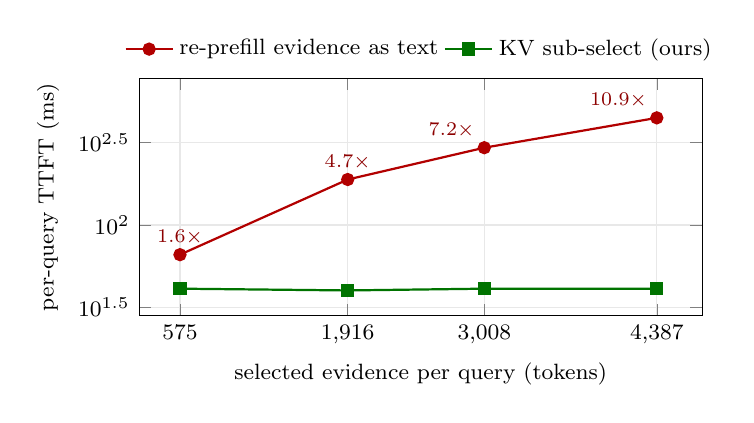
\begin{tikzpicture}
\begin{axis}[
  width=0.72\linewidth, height=4.6cm,
  xlabel={selected evidence per query (tokens)},
  ylabel={per-query TTFT (ms)},
  ymode=log, log basis y={10}, ymin=28, ymax=780,
  xmin=250, xmax=4750,
  xtick={575,1916,3008,4387},
  legend style={at={(0.5,1.03)}, anchor=south, legend columns=2, draw=none, font=\footnotesize},
  legend cell align=left,
  grid=both, grid style={gray!18}, font=\footnotesize,
  every axis plot/.append style={thick, mark size=2pt},
]
\addplot[red!70!black, mark=*] coordinates {(575,66)(1916,189)(3008,295)(4387,448)};
\addlegendentry{re-prefill evidence as text}
\addplot[green!45!black, mark=square*] coordinates {(575,41)(1916,40)(3008,41)(4387,41)};
\addlegendentry{KV sub-select (ours)}
\node[red!55!black,font=\scriptsize,anchor=south] at (axis cs:575,66) {$1.6\times$};
\node[red!55!black,font=\scriptsize,anchor=south] at (axis cs:1916,189) {$4.7\times$};
\node[red!55!black,font=\scriptsize,anchor=south east] at (axis cs:3008,295) {$7.2\times$};
\node[red!55!black,font=\scriptsize,anchor=south east] at (axis cs:4387,448) {$10.9\times$};
\end{axis}
\end{tikzpicture}
\caption{KV sub-selection decouples per-query latency from evidence size. As a query
selects more evidence, re-prefilling it as text grows TTFT ($66\!\to\!448$\,ms;
dense Qwen3-8B), whereas gathering the selected spans' KV re-prefills only the
question and stays flat ($\sim\!40$\,ms); the widening gap is the per-query speedup
(labeled, $1.6\times\!\to\!10.9\times$), reaching $32\times$ at $32$k selected tokens
(\S\ref{sec:eff}). First-token argmax matches the full-prefill oracle at every point.}
\label{fig:eff}
\end{figure}

\begin{table}[t]
\centering
\caption{KV sub-selection (``ours'') decouples the per-query \emph{prefill} from
the selected-evidence size: the sub-selected decode re-prefills only the question
(flat TTFT), while the text path re-prefills the evidence every query. Dense
Qwen3-8B; first-token argmax matches the full-prefill oracle at every row, and
end-to-end answers match the text path on this controlled synthetic set.}
\label{tab:eff}
\small
\begin{tabular}{lccc c}
\toprule
Selected / context (tok) & text tok/q & ours tok/q & TTFT (text $\to$ ours) & speedup \\
\midrule
0.6k / 3.2k  & 575  & 20 & $66\,\text{ms} \to 41\,\text{ms}$  & $1.6\times$ \\
1.9k / 4.3k  & 1916 & 20 & $189\,\text{ms} \to 40\,\text{ms}$ & $4.7\times$ \\
3.0k / 8.1k  & 3008 & 20 & $295\,\text{ms} \to 41\,\text{ms}$ & $7.2\times$ \\
4.4k / 13.5k & 4387 & 20 & $448\,\text{ms} \to 41\,\text{ms}$ & $10.9\times$ \\
\bottomrule
\end{tabular}
\end{table}

\paragraph{Cross-backbone robustness (non-Qwen).}
Position-preserving KV reuse is a property of the gather, not the weights, so we
expect it to hold on any RoPE model; we check one non-Qwen backbone rather than
claim architecture-independence outright. Re-running the correctness/efficiency
harness on \textbf{Llama-3.1-8B-Instruct}---a different architecture and
vendor---reproduces the guarantees on our test set: GATE-A/B first-token argmax
$6/6$ across $48$--$200$-step trajectories (residual $|\Delta\text{logit}|\le0.35$,
in fact \emph{tighter} than Qwen's $\sim\!0.7$), end-to-end match with text
re-prefill on all $6$ probes, and a \emph{flat} $\sim\!42$\,ms sub-select TTFT while
the trajectory grows $3.1$k$\to$$13$k tokens (the one-time prefill grows
$0.13\to0.52$\,s but amortizes), i.e.\ $2.8\times$ faster to first token at a fixed
selection. These are small-$n$ probes, not a broad multi-model study; the
per-query prefill decoupling from trajectory length holds on both
backbones we tested; the framework's \emph{accuracy} contribution is separately
evidenced across three benchmark families (\S\ref{sec:ama},
\S\ref{sec:locomo}, \S\ref{sec:lme}) rather than a single backbone.

\section{Related work}
\label{sec:related}

\paragraph{Agent-memory systems.}
The systems we compare to---AMA-Agent, Mem0~\citep{mem0},
MemoryBank~\citep{memorybank}, A-Mem~\citep{amem}, MemGPT~\citep{memgpt},
Zep~\citep{zep}, MemoRAG~\citep{memorag}, HippoRAG~\citep{hipporag}---share a
trait: they \emph{construct} memory at write time (extract facts, summarize, or
build graphs) and retrieve from that lossy store. AMA-Bench's own needle ablation
shows the cost: $-41\pp$ from lossy construction. Two precedents are closest to us.
\emph{Generative Agents}~\citep{genagents} retrieves by recency-importance-relevance
over a stream that mixes verbatim observations with summarized reflections, but
gives no verbatim-rehydration guarantee. \emph{MemGPT}~\citep{memgpt} pages
verbatim context via LLM tool calls but recursively summarizes overflow rather
than keeping it exactly rehydratable. \kvm{} differs by keeping raw spans as the
authoritative payload, routing to them, and serving gists only as a one-line
index and overview scaffold---never as a substitute for evidence a query needs,
which is always rehydrated verbatim.
Crucially, all of these are query-aware, so query-awareness is not the novelty;
the combination of \emph{verbatim payload} $+$ \emph{cheap routing} $+$
\emph{gist-as-index} is.

\paragraph{File- and transcript-based memory.}
A recent line of practice keeps raw history as-is and lets an agent search it
with tools: filesystem-backed agents over stored transcripts report strong
LOCOMO numbers~\citep{lettafiles,pamlocomo}, and AMA-Agent's tool loop over the
full trajectory JSON is the same idea on agent traces. These systems are
\emph{consistent} with our thesis---they, too, refuse to compress the
payload---and we do not claim priority on ``keep the raw text.'' Our
contribution relative to them is the controlled attribution (payload-fidelity
causality, the memory$\times$reader confound, structural addressing as a
separate channel) and the serving primitive (position-preserving KV
sub-selection), which text-file replay does not provide.

\paragraph{Retrieval-augmented generation and agent frameworks.}
Classic RAG retrieves external passages and conditions the reader on
them---RAG~\citep{rag}, REALM~\citep{realm}, RETRO~\citep{retro},
Atlas~\citep{atlas}. \kvm{} is RAG turned \emph{inward}: the corpus is the agent's
own trajectory and the retrieved units are re-injected as \emph{verbatim KV}
rather than re-encoded text, so retrieval and reuse share one representation
(the ``standard vector-RAG'' point of this design is our EmbeddingRouter,
\S\ref{sec:analysis}). The memory modules practitioners actually deploy---the
buffer/summary/vector stores in LangChain~\citep{langchain} and
AutoGen~\citep{autogen}---occupy exactly the slot \kvm{} targets; it is a
drop-in, verbatim-first alternative to those summary/vector defaults.

\paragraph{KV reuse and compression.}
A systems line reuses KV caches for latency---prefix caching in
vLLM~\citep{vllm} and SGLang~\citep{sglang}---which \kvm{} sits on top of. A
compression line removes tokens via eviction (e.g.\ H2O~\citep{h2o}) or learned
summarization (RECOMP~\citep{recomp}); these optimize the cache or the prompt,
not the \emph{selection-quality} memory question that determines whether a
multi-hop answer survives. A parallel architecture line compresses or retrieves
\emph{past activations} inside the model---Compressive
Transformer~\citep{compressivetransformer}, Memorizing
Transformer~\citep{memorizingtransformer}---whereas \kvm{} sits one level up, as a
training-free memory manager over the raw KV of a frozen model. Our point is
orthogonal and, where they overlap (at a
matched training-free, query-free budget), extractive retention is already at
least as good as generative summary---so the lever is selection, not harder
compression.

\section{Limitations: when does verbatim selection win?}
\label{sec:limits}

\kvm{} defers answer-extraction to the reader at inference time. This is ideal
for a capable, self-hosted reader and for dense/long-horizon evidence---where it
wins (AMA-Bench, LOCOMO). It has two boundaries. First, \emph{scope}: the
strongest form of our efficiency claim---position-preserving KV sub-selection of
arbitrary spans---needs self-hosting; hosted APIs expose only contiguous-prefix
prompt-caching, which our prefix-friendly layout still benefits from but which
cannot gather arbitrary spans. Second, \emph{reader capacity}: for a \emph{weak} reader over a
benchmark whose answers are tiny isolated facts, systems that extract atomic
facts at construction time can present an easier context---the gap is a matter of
reader capacity, not retrieval (our router surfaces the evidence $94\%$ of the
time). This is also why we report LongMemEval-S only in the strong-reader
(Qwen3-32B) regime: a scoping choice, testing the settings the claim is
about---capable self-hosted readers.

Third, \emph{once routing is strong, the reader is the residual bottleneck---and a
different answer-production paradigm owns one domain}. On AMA-Bench
\textsc{Software}, selection achieves $100\%$ recall of the asked steps, yet
AMA-Agent leads by $+17\pp$. The dissection in \S\ref{sec:ama} eliminates
retrieval, tool access, output format, and prompted iteration in turn; what
our reader lacks is the \emph{computational} step---code executed over the raw
trajectory to compute counts, diffs, and aggregations---plus AMA-Agent's
construction-time causal index. That is a genuinely complementary design, not
a retrieval gap, and our ablations indicate it cannot be absorbed by bolting
machinery onto a single-pass reader.

Fourth, \emph{verbatim storage has governance costs}. Unlike lossy construction,
the store retains raw history: PII persists verbatim and must be handled by
policy outside the memory (encryption at rest, retention windows, write-time
injection scanning---verbatim text stored is verbatim text replayed to the
reader). Deletion semantics differ by layer. In the \emph{text} substrate,
dropping a turn's segment is exact: the next assembly simply no longer contains
it, with no derived summaries or graph edges to chase down. In the \emph{KV}
layer it is not: cached keys/values are \emph{contextualized}, so the KV of
tokens \emph{after} an erased turn was computed while attending to it, and exact
erasure requires invalidating or recomputing the downstream blocks (bounded, in
our per-episode caches, by the episode length). We measured whether that
residue is \emph{extractable}: plant a secret credential at one step, erase
that step, and serve only later steps---either as KV gathered from the
full-trajectory prefill (carryover present) or as a compact re-prefill of the
same selected text (the secret information-theoretically absent). Asked
directly for the secret (Qwen3-8B, greedy, $40$ trials per condition), the
gathered-KV arm emitted it in $0/120$ trials at gap distances of $1/3/10$
steps, and the secret's first-token log-probability sat at the re-prefill
arm's noise floor ($\approx\!-31$ nats, within $1.1$ nats of an arm that never
saw the secret); a positive control that restates the secret in a
\emph{selected} step leaks in both arms ($120/120$ vs.\ $83/120$), so the
probe is sensitive. In this non-adversarial probe, carryover that is
measurable at the logit level did not surface erased content in
generation---but we still treat exact KV-layer erasure as requiring downstream
invalidation, make no claim under adversarial extraction, and have not
evaluated redaction pipelines.

\section{Conclusion}
\label{sec:conclusion}

For a long-horizon agent whose answers are exact, objective, and buried in a
dense trajectory---and whose history overflows the window or drowns the reader
in distractors---the right memory operation is to \emph{construct indices, not
answer payloads}: keep the raw history as reusable KV, index and scaffold it
cheaply, and rehydrate verbatim the spans a query needs. When the history fits
and the reader can exploit it, full context can win; when the reader is weak
and the facts are tiny, construction can win; we state both boundaries. Within
its regime, a small framework built on this principle leads our runs of
AMA-Bench (submitted for official verification), is competitive with dedicated
dialogue-memory systems on LOCOMO, and traces the selection-vs-full-context
crossover on LongMemEval-S, with the win driven by payload fidelity rather
than router sophistication, reader-side effects measured and reported
separately, and the cost amortized by KV reuse.
The recipe is simple enough to fork, and we offer it, with configurations and
predictions released, as a reproducible baseline that centers payload fidelity
over memory construction.

\section*{Reproducibility statement}
All code, configurations, the exact answer instructions
(Appendix~\ref{app:instr}), raw per-question predictions with judge scores for
every AMA-Bench run reported here (26 tagged runs, indexed by a results
manifest), the KV-equivalence and planted-secret probes with their outputs, the
analysis scripts that reproduce the bootstrap/cluster CIs and the step-pin
splits, and our leaderboard submission file are released at
\url{https://github.com/oklen/VeraKV}. AMA-Bench numbers come from the official
\texttt{run.py} harness with the memory plugged in through its method
interface; the structured answer instruction is a config-gated one-line swap,
disclosed and ablated in \S\ref{sec:analysis}.

\bibliographystyle{iclr2026_conference}
\bibliography{kvmemory_refs}

\appendix
\section{The three answer instructions, verbatim}
\label{app:instr}

The reader-side variable of \S\ref{sec:analysis} is a single swapped sentence.
For auditability we reproduce all three instructions exactly as run.

\paragraph{Default (harness).}
\begin{quote}\small
Provide a direct and concise answer.
\end{quote}

\paragraph{Structured (ours; $+5.1$--$5.8\pp$ at either router).}
\begin{quote}\small
Answer using ONLY the context above. Break the request into sub-questions if
needed, answer each citing exact evidence (values, step indices, outcomes)
VERBATIM, then give the final answer.
\end{quote}

\paragraph{Quote-first (probe; $-10.0\pp$ on \textsc{Software}, same batch).}
\begin{quote}\small
Answer using ONLY the context above. Locate the exact evidence first, then
answer by COPYING the exact strings from the context VERBATIM---commands, file
paths, code, values, error messages, step indices. Do not paraphrase or
re-describe them. The final answer should be the exact string(s) plus the
minimum wording needed to address the question.
\end{quote}

The comparison is itself a control: the structured and quote-first
instructions share the grounding preamble (``using ONLY the context above'')
and the same emphasis on verbatim evidence, and differ in what they ask the
reader's \emph{reasoning} to do---work through sub-questions versus copy
strings. The former gains $+5$--$6\pp$ overall, the latter loses $10\pp$ on its
probe domain: the structured instruction's value is the elicited sub-question
reasoning in the answering pass, not the grounding phrase or the verbatim
emphasis it shares with a losing variant.

\end{document}
